\documentclass[11pt]{article}
\usepackage[utf8]{inputenc}
\usepackage{geometry}
\usepackage{booktabs}
\usepackage{graphicx}
\usepackage{hyperref}
\usepackage{amsmath}
\usepackage{amssymb}
\usepackage{caption}

\title{Preferences in AI Project Report}
\author{Pratik Deshmukh}
\date{\today}

\begin{document}

\maketitle

\section{Introduction}
This report presents experiments on free-riding in sequential decision-making
under different \emph{statistical cultures}, following the framework of
\cite{lackner2023freeriding}. Our goal is to replicate the structure of Section~5
of that work while extending it with additional statistical cultures and updated
parameter settings.

\section{Background}

\subsection{Multi-Issue Model}
We study sequential decision-making in \emph{multi-issue elections}, where a set
of voters must decide on several issues, each with multiple candidates. Each
voter submits approval preferences for all candidates on each issue. A voting
rule is then applied issue by issue to determine the collective outcome.

\subsection{Voting Rules}
We focus on two major families of rules, following \cite{lackner2023freeriding}:

\begin{itemize}
    \item \textbf{Sequential Utilitarian Rule:} selects in each issue the
    candidate with the highest total number of approvals. This rule is
    equivalent to the mean OWA and is known to be immune to manipulation.
    \item \textbf{Thiele-Based Rules:} a general class where voter satisfaction
    decreases marginally as more of their approved candidates are selected.
    We evaluate sequential Thiele rules with parameters $x \in \{1,5,7\}$,
    where $x=0$ corresponds to utilitarian aggregation.
    \item \textbf{OWA-Based Rules:} aggregate voter satisfaction using Ordered
    Weighted Averages (OWAs). Following \cite{lackner2023freeriding}, we use
    normalized positive weights (no zeros) interpolating between utilitarian
    and leximin behavior. We evaluate parametric OWA rules with
    $x \in \{1,5,10,15\}$ and include an explicit \emph{leximin OWA} limit.
\end{itemize}

\subsection{Statistical Cultures}
The way preferences are generated strongly influences manipulation risks.
We consider four cultures:
\begin{itemize}
    \item \textbf{p-IC}: per-issue impartial culture, sampling approvals
    independently with probability $p=0.5$.
    \item \textbf{Disjoint Groups}: voters are divided into $g=2$ groups with
    internally aligned preferences.
    \item \textbf{Resampling Model}: preferences are generated by resampling
    with parameters $(p, \phi) = (0.5, 0.5)$ controlling randomness and correlation.
    \item \textbf{Hamming Noise}: preferences are first generated from another
    culture and then perturbed by flipping approvals with small probability
    $\epsilon=0.1$ per issue. This noise model captures robustness under
    small random perturbations.
\end{itemize}

\subsection{Free-Riding Notion Used in the Experiments}
We adopt the paper’s definition and apply the following operationalization:
(i) a voter can attempt to free-ride on issue $i$ only if she \emph{originally
approved the winning candidate} on $i$; (ii) to test manipulation, we replace
the ballot on issue $i$ by a \emph{restricted} deviation that drops that single
approval (all other approvals are kept fixed), and we require that the winner on
issue $i$ \emph{remains unchanged} (the voter is non-pivotal on $i$); (iii) the
election outcome is recomputed using the manipulated profile, but the voter’s
gain/loss is assessed with her \emph{truthful} utilities.
This deviation class is a subset of all free-riding deviations discussed in
\cite{lackner2023freeriding} but is sufficient for our experiments.

\subsection{Risk Metrics}
We evaluate manipulation opportunities using the following metrics:
\begin{itemize}
    \item \textbf{Trials:} total number of voter–issue pairs considered ($n \times k$).
    \item \textbf{Eligible:} \# pairs where the voter originally approved the winner.
    \item \textbf{Possible:} \# eligible pairs where dropping that single approval leaves the winner unchanged.
    \item \textbf{Successes:} \# possible pairs where the voter’s truthful utility increases.
    \item \textbf{Harms:} \# possible pairs where the voter’s truthful utility decreases.
    \item \textbf{Success rate:} $\text{successes} / \text{trials}$.
    \item \textbf{Harm rate:} $\text{harms} / \text{trials}$.
    \item \textbf{Risk:} $\text{harms} / \text{possible}$ (conditional probability of harmful manipulation).
\end{itemize}

\section{Methodology}
We replicate the experiments from Section~5 of \cite{lackner2023freeriding},
using four statistical cultures: impartial culture (p-IC), disjoint groups,
the $(p, \phi)$-resampling model, and the Hamming-noise model. For each culture,
we run multiple random seeds and compare risk metrics under sequential
utilitarian, sequential Thiele rules ($x=1,5,7$), and OWA rules ($x=1,5,10,15$, plus leximin).

\subsection{Parameters}
The main parameters used in our experiments are:

\begin{itemize}
    \item Number of voters: $n=20$
    \item Number of issues: $k=5$
    \item Candidates per issue: $c=4$
    \item Random seeds: $200$
    \item Cultures and hyperparameters: as defined above.
\end{itemize}

All configurations were executed using a unified experimental pipeline,
which produces both tabular summaries and risk plots.

\section{Results}
The combined results table is automatically generated by the experiment
pipeline. The table below is included directly from the output file:

\begin{table}[h!]
\centering
\resizebox{\textwidth}{!}{%
\input{tables/combined.tex}
}
\caption{Combined results across cultures and rules. Risk metrics include trials,
eligible, possible, successes, harms, success/harm rates, and risk
(defined as harms/possible).}
\label{tab:combined}
\end{table}

\subsection{Per-Culture Comparisons}
To visualize the trends, we show manipulation risks by rule family (Thiele and OWA)
for each statistical culture.

\paragraph{p-IC.}
\begin{figure}[h!]
\centering
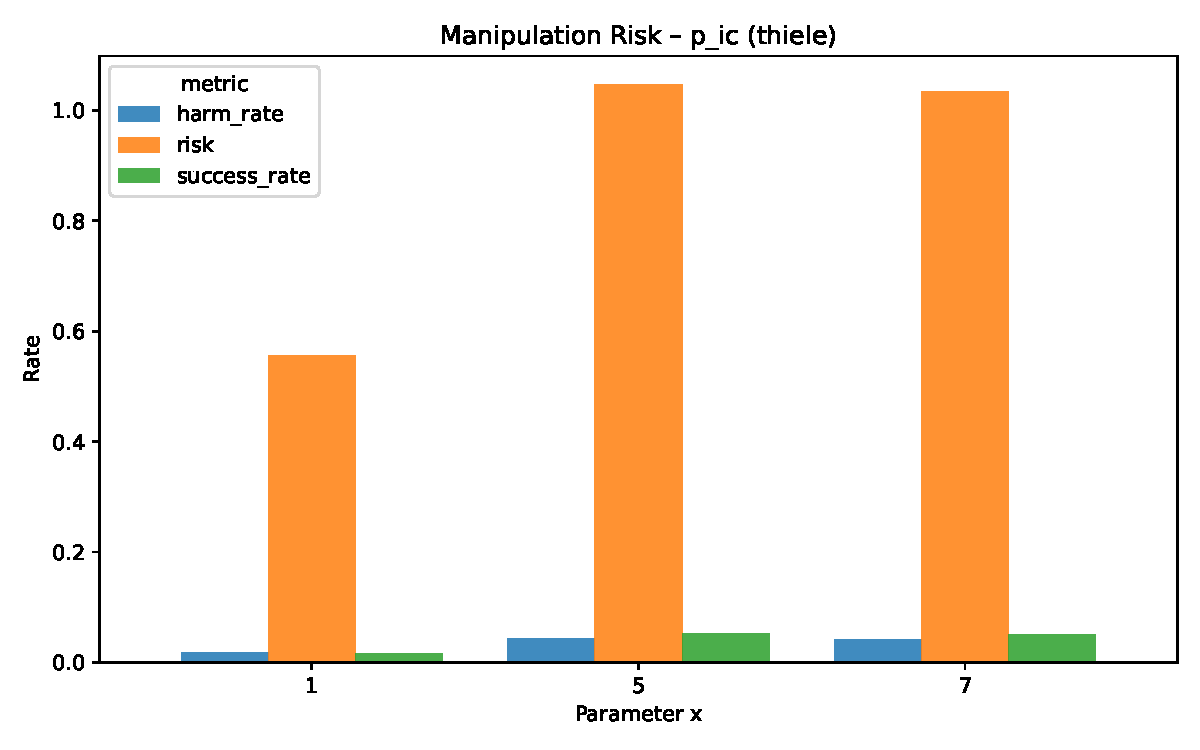
\includegraphics[width=0.7\textwidth]{figures/risk_p_ic_thiele.pdf}
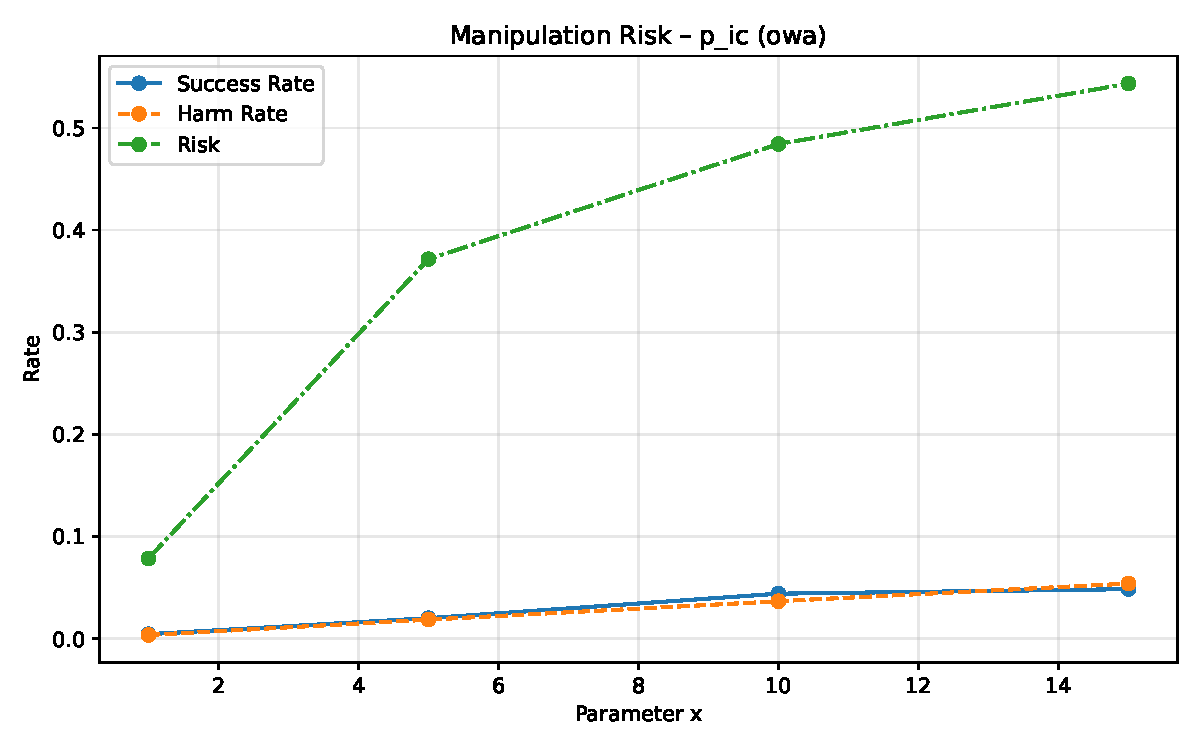
\includegraphics[width=0.7\textwidth]{figures/risk_p_ic_owa.pdf}
\caption{Manipulation risk under p-IC culture. Top: Thiele rules. Bottom: OWA rules.}
\end{figure}
Under p-IC, the utilitarian rule is immune (zero across all metrics). Within Thiele and
OWA families, success rates are small but increase with the family parameter $x$; harms
remain tiny, and risk (harms/possible) is near zero. In our runs, the leximin extreme
shows the largest success within OWA, consistent with the trend that moving away from
utilitarian slightly increases exploitable opportunities.

\paragraph{Disjoint Groups.}
\begin{figure}[h!]
\centering
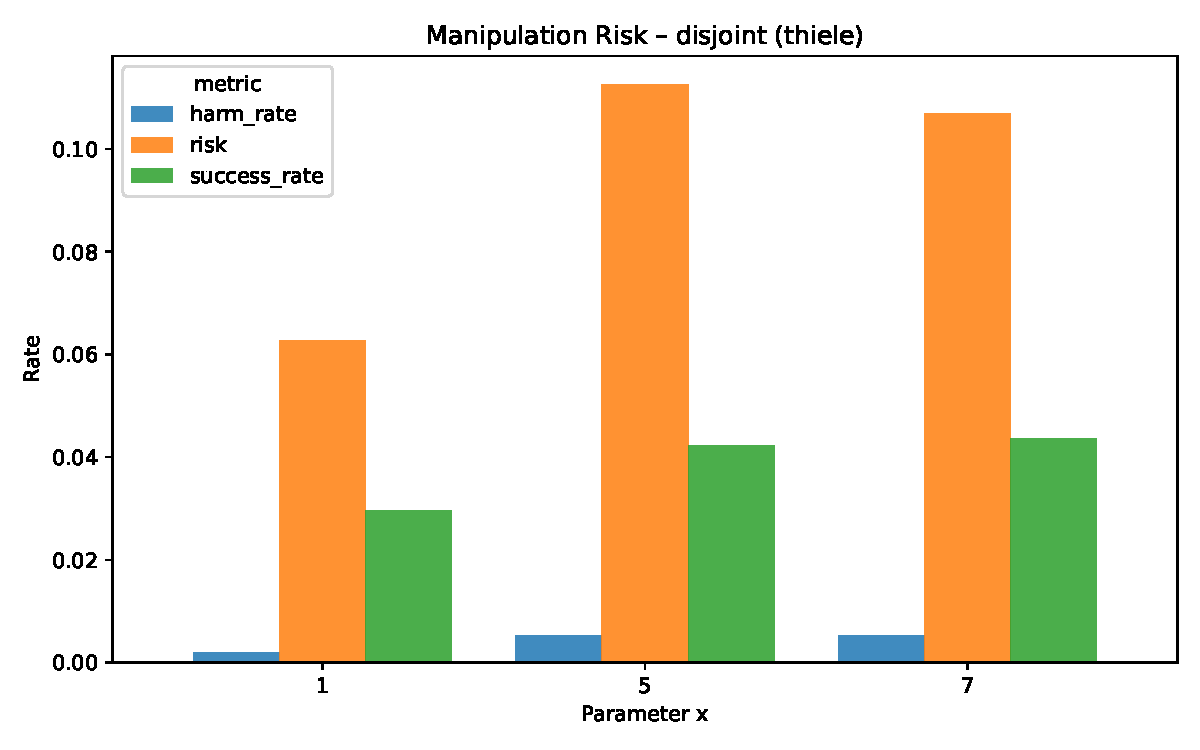
\includegraphics[width=0.7\textwidth]{figures/risk_disjoint_thiele.pdf}
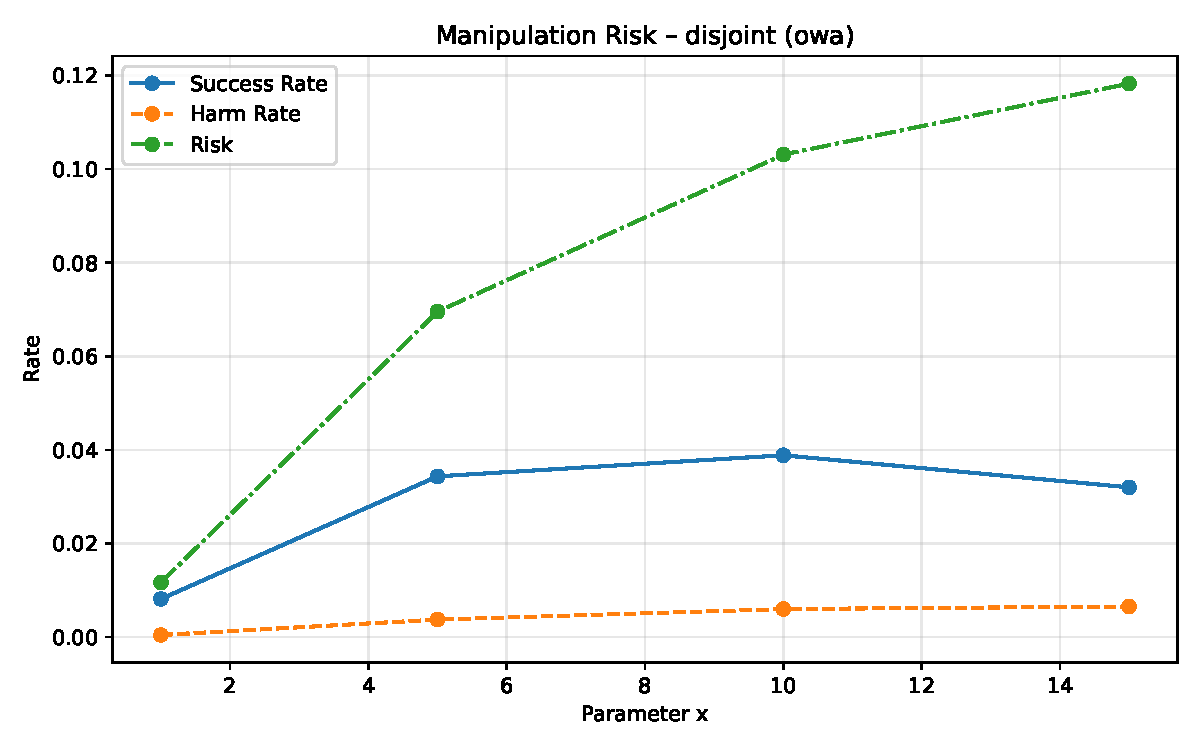
\includegraphics[width=0.7\textwidth]{figures/risk_disjoint_owa.pdf}
\caption{Manipulation risk under disjoint-group culture. Top: Thiele rules. Bottom: OWA rules.}
\end{figure}
Correlated group structure reduces overall opportunities compared to p-IC. Success
rates remain low across both families; harms are close to zero and risk is negligible.

\paragraph{Resampling Model.}
\begin{figure}[h!]
\centering
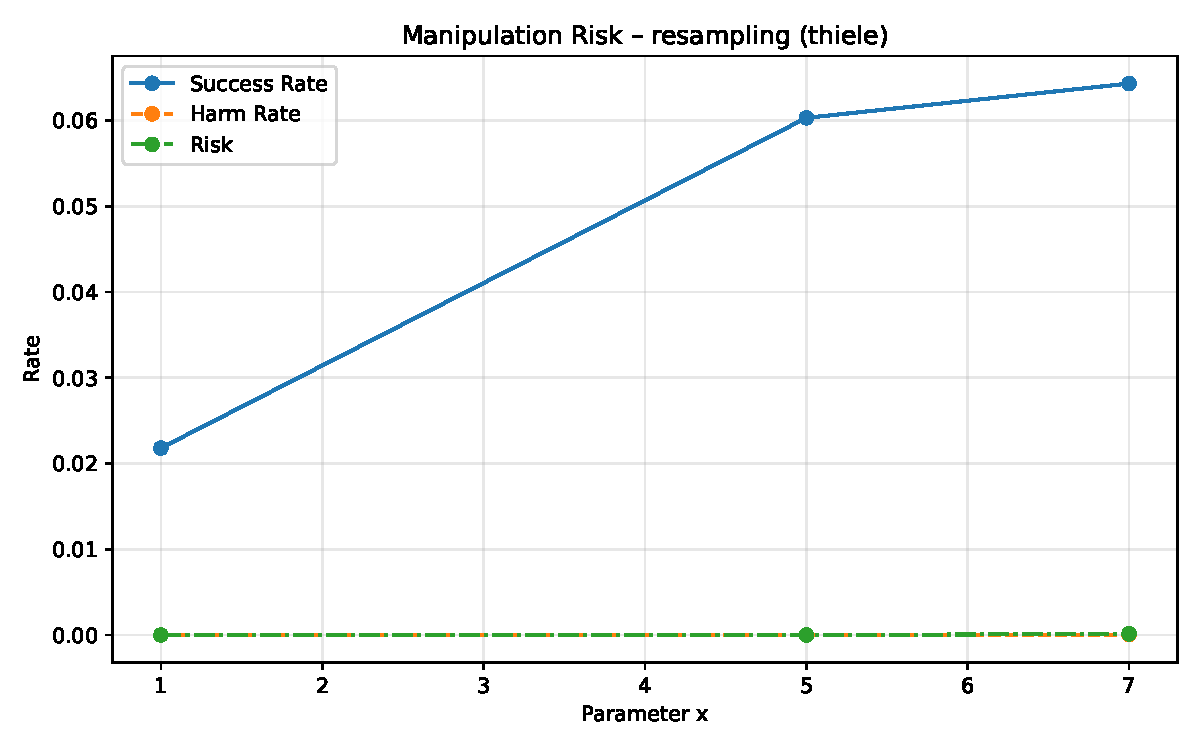
\includegraphics[width=0.7\textwidth]{figures/risk_resampling_thiele.pdf}
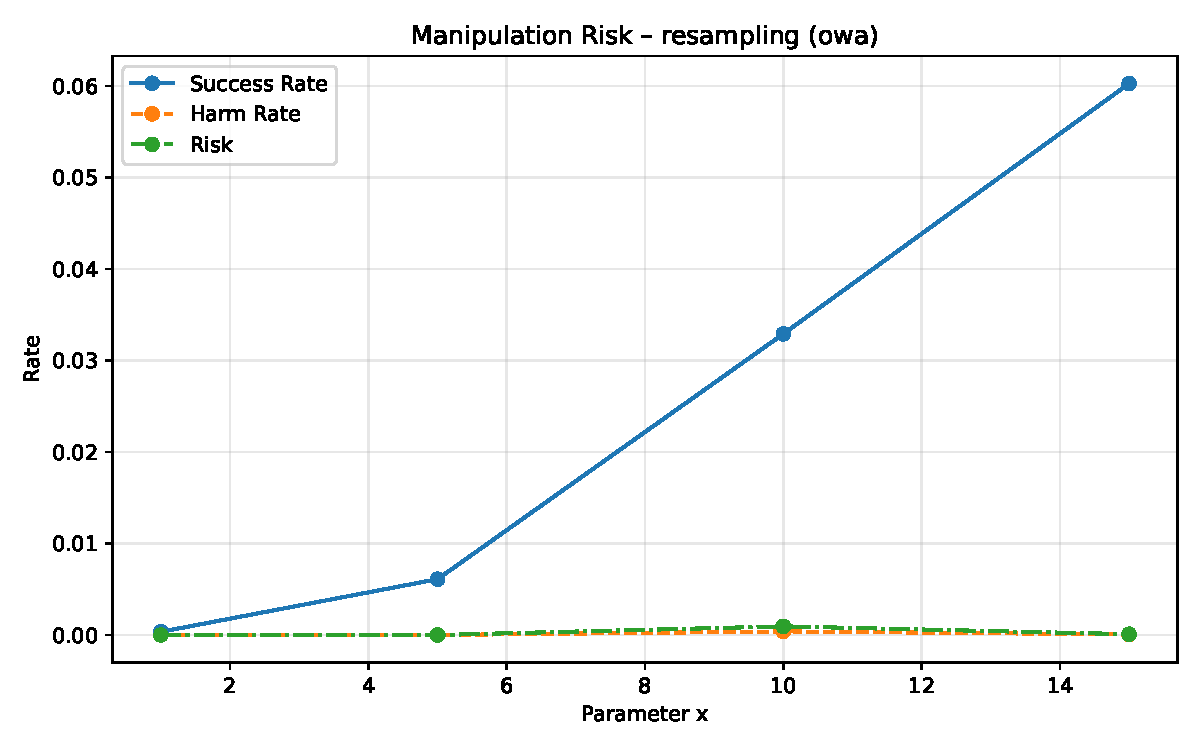
\includegraphics[width=0.7\textwidth]{figures/risk_resampling_owa.pdf}
\caption{Manipulation risk under resampling culture. Top: Thiele rules. Bottom: OWA rules.}
\end{figure}
Resampling yields patterns similar to p-IC: utilitarian is immune; success rates increase
modestly with $x$ in both families; harms and risk remain very small.

\paragraph{Hamming Noise.}
\begin{figure}[h!]
\centering
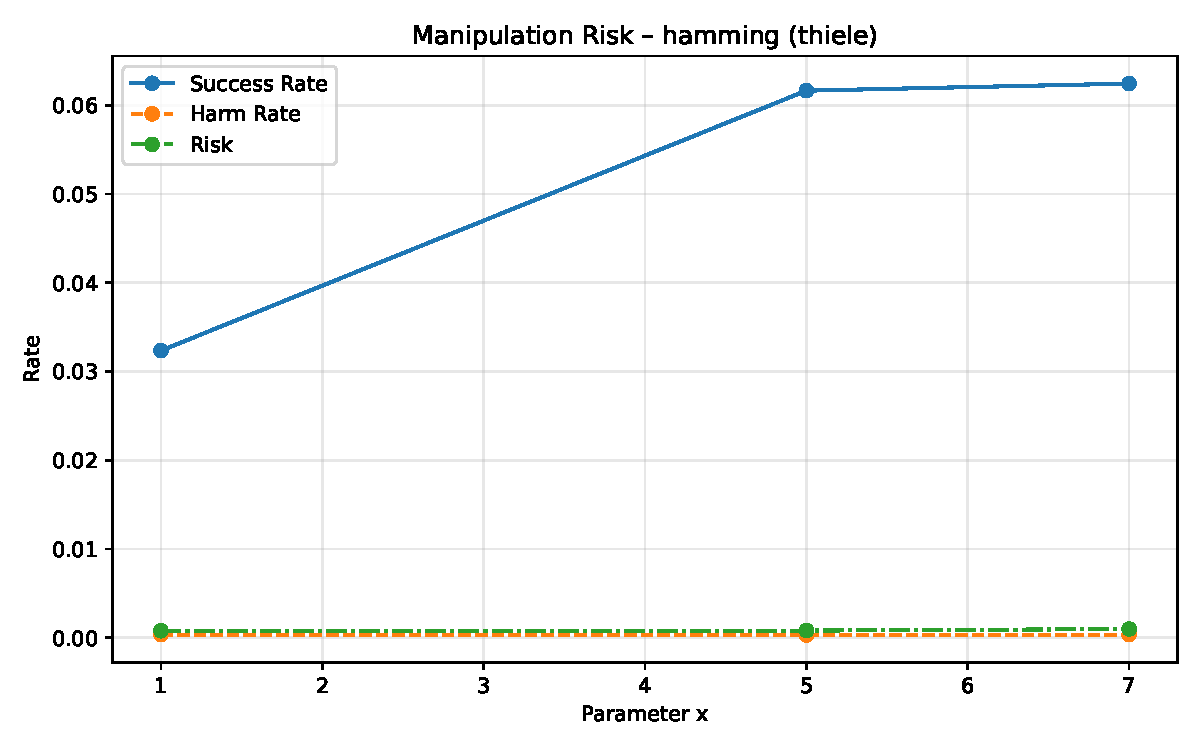
\includegraphics[width=0.7\textwidth]{figures/risk_hamming_thiele.pdf}
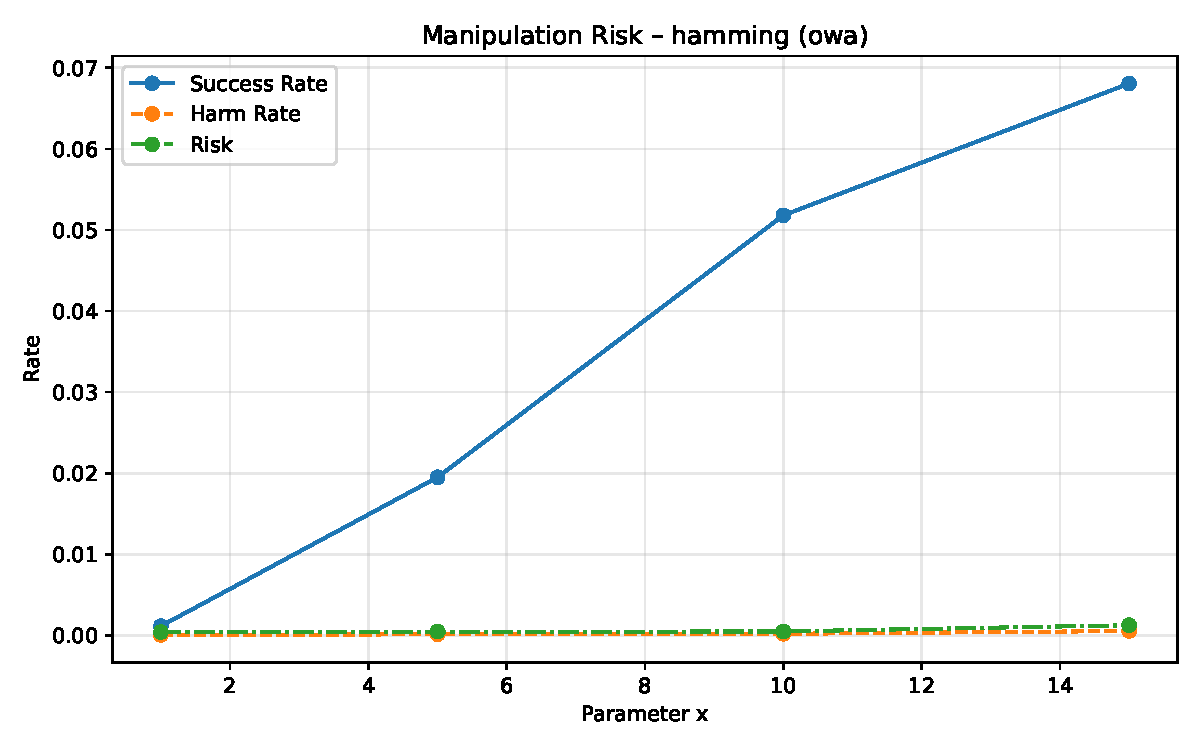
\includegraphics[width=0.7\textwidth]{figures/risk_hamming_owa.pdf}
\caption{Manipulation risk under Hamming-noise culture. Top: Thiele rules. Bottom: OWA rules.}
\end{figure}
Noise adds mild random perturbations but preserves the qualitative trends:
utilitarian stays immune; success rises slightly with $x$; harms and risk remain
near zero.

\section{Discussion}
Our experiments highlight the dependence of manipulation risk on both the
voting rule and the statistical culture.

\paragraph{Effect of Statistical Cultures.}
The \emph{p-IC} and \emph{resampling} cultures show modest manipulation opportunities.
The \emph{disjoint} model has fewer opportunities overall. \emph{Hamming noise} perturbs
preferences slightly but does not qualitatively change the picture.

\paragraph{Effect of Voting Rules.}
The \emph{utilitarian rule} (equivalently mean OWA) is immune to manipulation.
For both Thiele and OWA families, moving away from the utilitarian endpoint
(flarger $x$ in our parameterization) increases the fraction of successful free-rides,
while harm remains rare; consequently, risk (harms/possible) stays very small.

\paragraph{Risk Metrics.}
Across all settings, harms are rare relative to both trials and possible cases,
and the risk measure (harms/possible) is consistently close to zero.
Taken together, manipulators succeed more often than they harm themselves under
the restricted deviation class we test.

\section{Conclusion}
The choice of statistical culture influences the frequency of free-riding
opportunities, but the qualitative ranking across voting rules is stable in our
experiments. Utilitarian is immune; within Thiele/OWA families, higher~$x$ values
show somewhat more manipulability, yet harms remain rare and risk is small.
These findings are compatible with the trends discussed by \cite{lackner2023freeriding}
under our (restricted) deviation model.

Future work could extend these experiments by exploring richer parameter grids
for $(p,\phi)$ and $\epsilon$, by scaling to larger electorates, and by testing
the full family of admissible free-riding deviations described in
\cite{lackner2023freeriding} (beyond single-approval drops).

\section*{Repository}
The full project code and report sources are available at: \\
\href{https://github.com/inquisitour/preferences-in-ai}{github.com/inquisitour/preferences-in-ai}

\bibliographystyle{plain}
\bibliography{references}

\end{document}
% !TEX root = report.tex
